\documentclass[a4paper]{IEEEtran}
\usepackage{hyperref}
\usepackage{url}
\usepackage{graphicx}

\begin{document}
\author{Catalin David}
\title{Channel Modelling Using Bellhop in Underwater Acoustic Sensor Networks}

\maketitle
\begin{abstract}
In this paper we describe a step by step procedure on how to experiment and
evaluate the Bellhop model.
\end{abstract}

\section{Introduction}
Studying and modelling how underwater sensor networks behave is a new and
difficult task, but the rewards are incredible: exploration of the ocean which
covers about 70\% of the earth surface -- this will ease the search of new
energy sources, it will allow environmental and industrial monitoring (of
animals and equipment), early disaster warning (for earthquakes, tsunamis) and,
of course, for other military purposes.

While the design of such a system might seem related to the one of terrestrial
networks, it is very different. Unlike the terrestrial counterpart, for
underwater networks only acoustic communications are considered to be viable (at
the physical layer) and this creates issues, since in the terrestrial setting
you have radio frequency (RF) communications. In an underwater environment, RF
has been tested and the results were not very good, the transmission suffering
from severe atenuation, the only succesful deployment being at very low
frequencies and with a large antenna and a very high transmission power. Still,
this is not what one would have in mind when thinking about an underwater sensor
network: an underwater sensor network consists of many interlinked sensors that
are deployed once and with which there is no physical interaction for a long
period of time. This generates many requirements, but the most important for the
networking part are energy efficiency and a reliable transmission, leading to
the study of acoustic channels.

From a networking point of view, the acoustic communication is very different
from the RF communication, mainly due to the low bandwidth, propagation delay
and the quality of the link. One other important thing to note is that
underwater networks are, in general, very prone to noise due to the environment
-- waves, shipping activity, a modification in the temperature or salinity of
the water etc. We consider now a network with multiple nodes in which there
might be multiple paths between each destination and receiver. If terrestrial
protocols were to be used in such a volatile environment, when a link would be
down, there would be an increased amount of traffic in the network for rerouting
the transmission of data, leading to a high energy usage, ignoring one of the
main requirements.

Since the development and deployment costs for such a network, alognside with
the limited remote access to the deployed network,  one of the challenges
involved is to develop a valid simulation model that is able to provide results
that are according to real life. Once that is done, one can experiment with
different theoretical implementations and find out more about the underwater
communication constraints and limits.

\section{Background}
\subsection{Motivation}
In order to deploy an underwater network, one needs both financial and time
resources, as it is a very expensive and difficult task. Therefore, prior to the
deployment of such a network, all efforts need to be made in order to find new
ways to deal with the challenges of such an environment. This motivates
researchers to find models that try to simulate as well as possible the
conditions of the seabed (where the network will most likely be deployed).

Some of the challenges found in the underwater environment are long latency and
limited bandwidth, a high degree of noise, high bit error rates and transmission
loss, reliability, energy and cost constraints, as well as volatile link
quality. A few of these are briely explained below.

\textit{Long Latency and Limited Bandwidth}: The acoustic channel in the
underwater environment is characterized by long latency and limited bandwidth.
The speed of propagation of acoustic waves ($1.5 x 10^3 m/s$) is five orders of
magnitude lower than the one specified for an RF environment. For this, we need
to consider the propagation range, which can vary between few meters and many
kilometers. In any case, the bit rate for such a channel is very low.

\textit{Noise, High Bit Error Rates and Transmission Loss}: The underwater
environment is subject to a lot of noise coming from different sources, such as
turbulences, wind, shipping activity and thermal effects, as well as seismic
activity, fishes swimming. The model has to be very elastic with regards to all
these factors which, in real life, can actually produce communication failure
over certain links. Even without noise, a model has to take into consideration
the attenuation (transmission loss) of the signal, which increases with both
distance and frequency, as well as geometric spreading.

\textit{Energy and Cost Constraints}: Deploying a network of underwater nodes is
much more complicated than deploying the same network in the terrestrial
environment. The biggest constraints are that in the underwater environment, the
node casing has to resist a great pressure and that the nodes should be
independent of human activity (it is costly to take out and put back the nodes
every day). Moreover, light sources are not available at such depths, resulting
in a system that has to be very energy efficient. Coupling that with such a bad
channel quality, in which the communication protocols might fail, which results
in retransmission, we get a very high amount of used energy.

As previously noted, all these factors, all these constraints motivate people to
try even more to find new ways to communicate underwater, to better understand
the transmission specifics for this environment, to develop new technologies and
models before committing to actually deploying such a network.

\subsection{Previous Work}
As stated before, the need for understanding the characteristics of
communication in an underwater channel is one of the basic prerequisites in
order to create better underwater sensor networks. Still, the experiment
conducted does not focus on a general approach towards modelling the entire
environment, but we are focusing on a specific region (near the bottom of the
sea). The experiment in this article is based on real data (fed into the Bellhop
modelling tool \cite{bellhop}) and tries to be as close to reality as possible,
by using multipath for signal analysis -- which is relevant since we are talking
about the bottom of the sea where reflections from the seabed are possible.

The work of M. Stojanovic \cite{stojanovic} is very relevant to this field, as
it documents the theoretical background behind underwater channel analysis. This
article synthesises the required mathematical background, as well as channel
analysis knowledge. Since this article is of high relevance in the field and is
acknowledged to be one of the best, this allows us to use the theory and
calculations documented to reach the desired results.

The purpose of the experiment is to reproduce the results provided by
\cite{book} so that they can be used later on in the related paper: \cite{nds}.
We base our experiment on the data from the article. Relevant work is also
documented in \cite{hayward}, where the authors also try to determine the
channel characteristics (bandwidth and channel capacity), but unlike the work
documented here, their research is based on communication links in the upper
half of the water column.

An alternative to using a ray-tracing algorithm such as Bellhop is to use the
NS-2 simulator and extend it to adjust to the underwater environment. Such a
model has been implemented, by extending the NS-2 simulator (see \cite{ns2}) and
has provided great results, with a very small amount of used computation time.
Still, due to the nature of the simulator, the data is not similar to the one
obtained from a ray-tracing algorithm, since NS-2 uses a single path from source
to destination (similar to a water rippling effect), while a ray-tracing
algorithm provides multipath and a more in-depth analysis of the data (one can
find out the exact path that the ray went through to reach the destination, the
phase shift of the signal and how it contributes to the final impulse response).

\section{Methodology}
A number of steps need to be taken in order to achieve the results. First of
all, data that describes the environment needs to be collected. This data is
then transformed to a computer-understandable format for the modelling tool
(Bellhop program) to understand it. Then the modelling tool interprets this data
and runs, generating the output. This output will then have to be postprocessed
in order to compute the channel characteristics. Since we are committed to using
the Bellhop program for ray-tracing, part of the Ocean Acoustic Library
\cite{oal}, we will describe the process in a detailed way for this modelling
tool. Still, if one wishes, another modelling tool can be used, but this will
have impact with regards to the preprocessing and postprocessing of the data
(but the general workflow will be the same.

\subsection{Preprocessing the Environment}

The Bellhop program uses as input environment files (usually with extension
ENV). An environment file serves as a description of how the environment behaves
at certain parameters, as well as to instruct the Bellhop program what output
data is required, in what format the data will be output, all according to a
certain template. The environmental file comprises of a few ``sections'' that
describe characteristics of the environment, such as sound speed profile and
bathymetry. These sections of environmental file are presented below in theory,
as well as as how they look in our model, in section \ref{sec:case}.

\subsubsection{Frequency}
One constraint (or feature) of the Bellhop tool is that it can only use one
frequency at which it operates. Therefore, in order to perform a multi-frequency
analysis, one must define multiple input files, one for each frequency. The
start, end and step frequency are to be determined by the user, depending on the
use and wished granularity of the output. The main impact of this paramater is
over the transmission loss (or attenuation) of the signal, as this higly
dependant on the frequency in an underwater environment.

\subsubsection{Sound Speed Profile}
Since we are using acoustic waves and an inhomogeneous propagation environment,
this system has to obey Snell's law of propagation: $$ \frac{\cos{\theta}}{c} =
constant $$

This means that the acoustic rays will not travel in a straight line, but they
will bend towards the areas of lower speed. This data can be generated, but it
is better if this data actually comes from real measurements near the
area of interest. In general, the speed of sound is not revealed by
measurements, but it is described in term of other measurements by the
following equation: 
\begin{eqnarray*}
 c = 1449.2 + 4.6 T - 0.055 T^2 + 0.00029 T^2 +\\
(1.34 - 0.01 T)(s - 35) + 0.06z
\end{eqnarray*}
where $T$ stands for temperature (in Celsius degrees), $s$ is salinity
in Practical Salinity Units (PSU) and $z$ is the depth (meters).
Therefore, in order to find the speed of sound at different depths, we
only need the salinity and temperature measurements for a certain
area. These values can usually be obtained via the Bedford Institute
of Oceanography (BIO) \cite{bio} or via the National Oceanic and
Athmospheric Administration (NOAA) \cite{noaa}. Still, these values
are not stable, as the temperature might vary during the day, month, season or
year, so the SSP must be generated either from averaged values for these
parameters or the SSP can be specific to a certain time, case in which
one would only take into consideration a specific scenario.

\subsubsection{Bottom Description}
In our modelled scenario, we have an interest in sound propagation
near the bottom of the sea. Since we are using the Bellhop program
which performs ray-tracing, thus taking into consideration multiple
paths between the source and the destination, we need to provide the
program a description of the seabed. The description must be given in
terms of three components: how the sound propagates through the
seabed, how rough is the terrain and what is the bathymetry of the
region of interest.

The first option refers to the way acoustic rays interact with the
seabed. The seabed can be considered to be a vacuum-like surface
(sound does not propagate through), a perfectly reflective surface or
it can have a more complicated description.

The roughness of the terrain is given as a root-mean-squared (RMS)
value in meters of the inter-facial features of the sea bottom. The
last parameter is the actual bathymetry of the seabed -- this has to
be provided in an additional file (BTY), one per each ENV file
corresponding to a single direction.

\subsubsection{Sources, Receivers, Ranges}
In the ENV file, multiple sources, multiple receivers and multiple
ranges can be specified. Ray-tracing is performed between only a
sender and a receiver, each of which is characterized by a depth and
the entire system is characterized by a distance between the
nodes. Using Bellhop, we can specify multiple depths for the sources,
multiple depths for the receivers and multiple distances between the
sender and receiver, meaning that ray-tracing can be computed
for multiple $\langle source,receiver,range \rangle$ tuples. Since
ray-tracing is performed for each of these tuples, that means there
are $$\#sources \times \#receivers \times \#ranges$$ possibilities for which the
program must be run, thus yielding a direct proportionality between each of
the number of sources, receivers and ranges and the final runtime of
the program.

\subsubsection{Run Type}
The Bellhop program is designed with many options with regards to the
type of computations that it can perform and also with regard to the
type and format of the output. There are three main types of output
that Bellhop can provide: ray, amplitude-delay and acoustic field.

Ray files contain the exact path of the rays that travel between the
source and the destination. The amplitude-delay files contain
information about each ray that travels between source and destination
in terms of strength, phase shift and delay at the destination. The
last type, acoustic field is used to describe the ocean as an actual
acoustic field in which the most important information is the relative
signal strength within the desired area. For this experiment, we are
interested in the amplitude-delay output of Bellhop.

\subsubsection{Beam Width}
In order to limit and reduce the number of rays for which the path
must be calculated, we can impose a restriction at the source on how
wide the beam should be. This can be done by providing a minimum and
maximum angle between which the rays can start propagating from the
source. The values for these angles can be both negative, case in
which this is an angle towards the surface of the water, or
positive, case in which this is an angle towards the bottom. Besides
these angles, we can also provide the number of beams that will start
from the source within this range or we can let Bellhop decide what
the best value is.

\subsubsection{Bounding Box}
Ray-tracing is a very time and processor-intensive operation,
therefore, a bounding box has been introduced to further reduce the
amount of rays that can be followed. Still, if a too small bounding
box is used, this can interfere with the ray-tracing algorithm (as
some of the rays exit the bounding box), so the recommended bounding
box should extend slightly behind the bottom depth and behind the
maximum range.
\subsection{Arrival Analysis and Data Interpretation}

\subsubsection{Arrival file analysis}
\subsubsection{Channel Response analysis}
\subsubsection{Noise analysis}
\subsubsection{Signal to noise ratio}
\subsubsection{Bandwidth}
\subsubsection{Capacity}

\section{Case Study}
\label{sec:case}

\subsection{Preprocessing}
%% env files
%% SSP -- table with values
%% Bathymetry -- make plot
%% Run Type
%% Beam Width
%% Bounding box

\subsection{Bellhop processing}

\subsection{Postprocessing}
%% Arrival file analysis -- plot signal strength
%% Noise analysis -- plot noise
%% Signal to noise ration -- plot sig2noise
%% Bandwidth -- plot bw
%% Capacity -- plot capacity

\subsection{Range based evaluation}
%% varying the range -- how does it affect the bandwidth and capacity

\subsection{Depth based evaluation}
%% varying the depth of the nodes -- how does it affect the bandwidth and
%%capacity
\begin{figure}
\centering
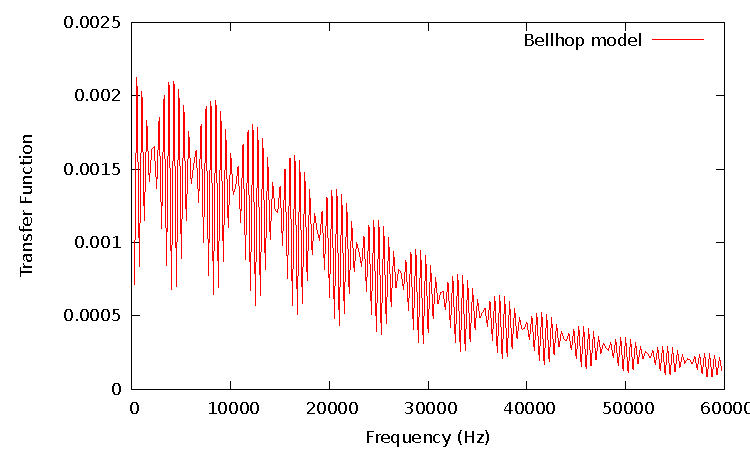
\includegraphics[width=3.5in]{../postprocessing/hreal00.pdf}
\end{figure}

\begin{figure}
\centering
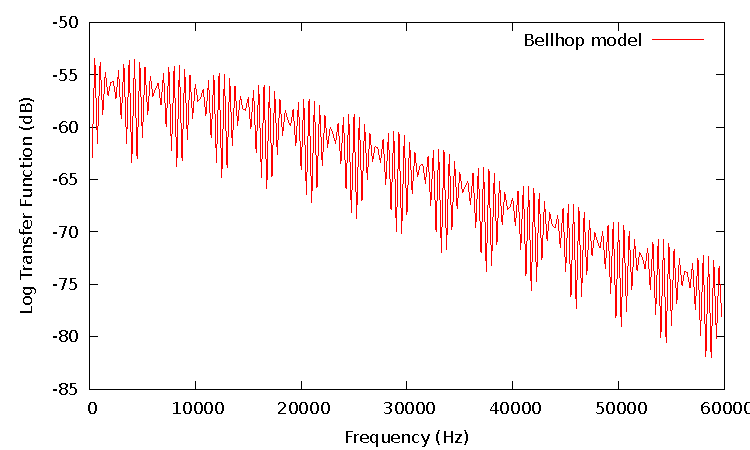
\includegraphics[width=3.5in]{../postprocessing/logh00.pdf}
\end{figure}

\begin{figure}
\centering
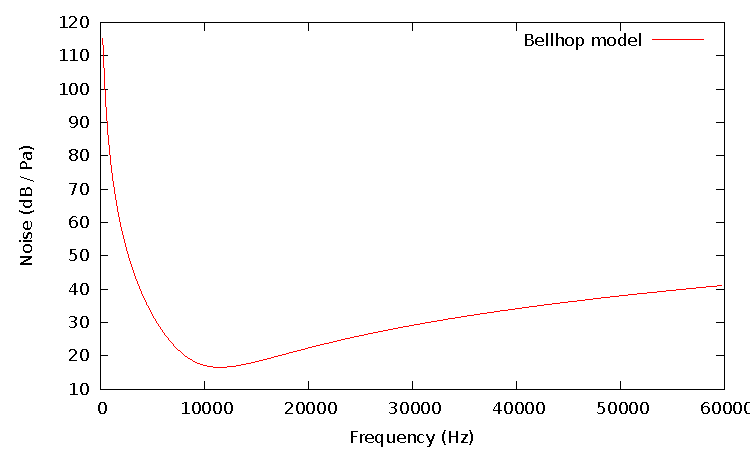
\includegraphics[width=3.5in]{../postprocessing/noise00.pdf}
\end{figure}

\begin{figure}
\centering
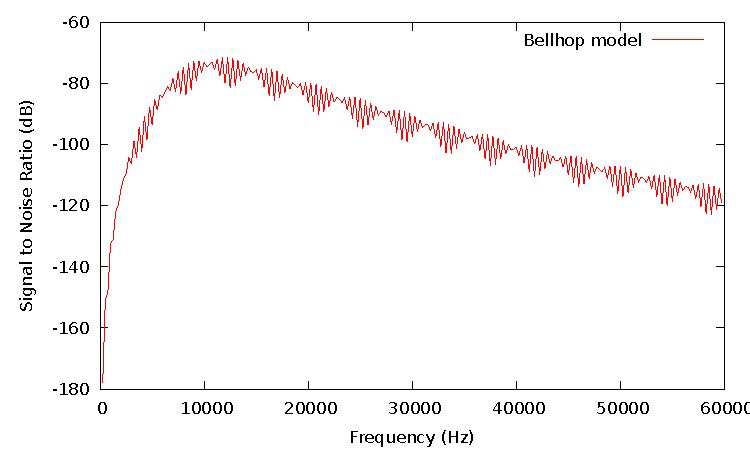
\includegraphics[width=3.5in]{../postprocessing/sig2noise00.pdf}
\end{figure}

\begin{figure}
\centering
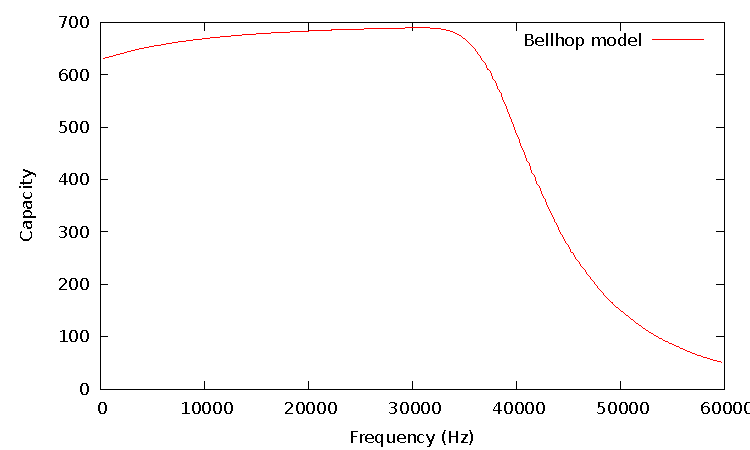
\includegraphics[width=3.5in]{../postprocessing/capacity00.pdf}
\end{figure}

\begin{figure}
\centering
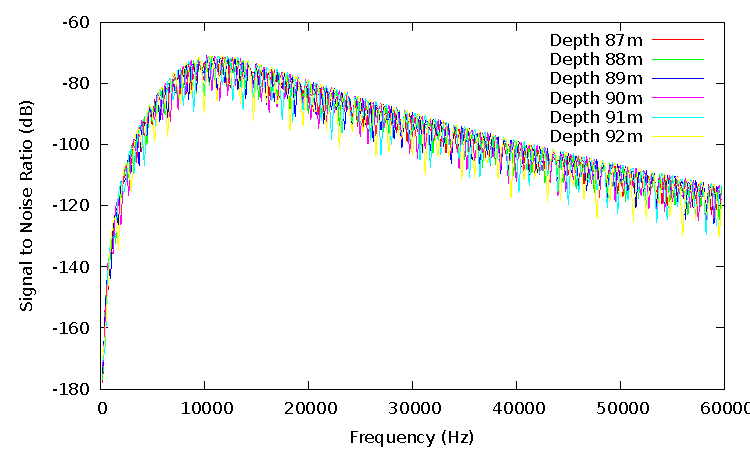
\includegraphics[width=3.5in]{../postprocessing/sig2noiseDepth.pdf}
\end{figure}

\begin{figure}
\centering
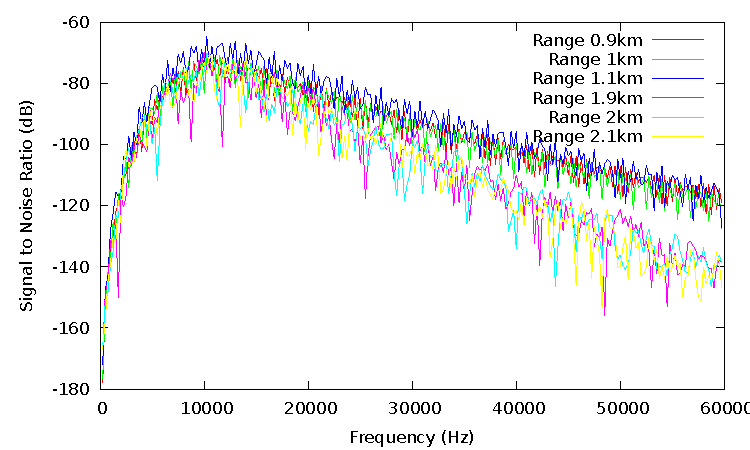
\includegraphics[width=3.5in]{../postprocessing/sig2noiseRange.pdf}
\end{figure}

\begin{figure}
\centering
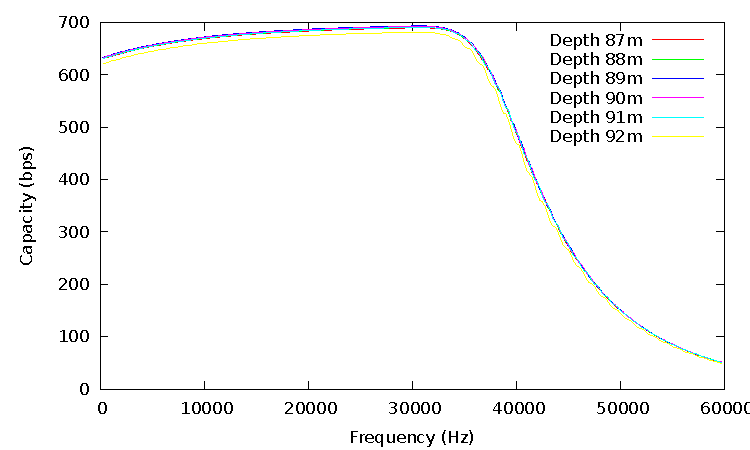
\includegraphics[width=3.5in]{../postprocessing/capacityDepth.pdf}
\end{figure}

\begin{figure}
\centering
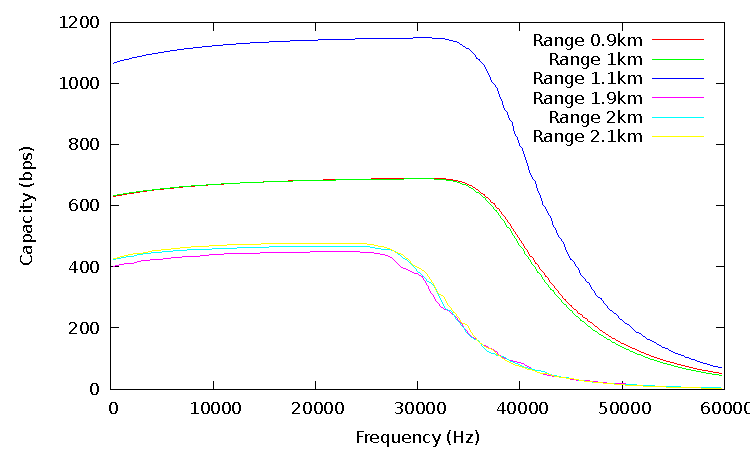
\includegraphics[width=3.5in]{../postprocessing/capacityRange.pdf}
\end{figure}

\section{Future Work and Conclusion}

\begin{thebibliography}{99}
\bibitem{capacity} \textit{A study of channel capacity for a seabed underwater
acoustic sensor network}, Peter King, Ramachandran Venkatesan, Cheng Li
\bibitem{model} \textit{An Improved Communications Model for Underwater Sensor
Networks}, Peter King, Ramachandran Venkatesan, Cheng Li
\bibitem{book} \textit{Channel Modelling for Underwater Acoustic Sensor
Networks}, Peter King, Ramachandran Venkatesan, Cheng Li -- Chapter 12 in
Underwater Acoustic Sensor Networks, Edited by Yang Xiao
\bibitem{nds} \textit{A Comparison of Channel Models for Simulating Underwater
Acoustic Communications}, Anuj Sehgal, Catalin David, J\"urgen Sch\"onw\"alder
\bibitem{stojanovic} \textit{On the Relationship Between Capacity and Distance
in an Underwater Acoustic Communication Channel}, Milica Stojanovic
\bibitem{bellhop} \textit{General description of the BELLHOP ray tracing program
(June 2008 release)}, Orlando Camargo Rodriguez
\bibitem{hayward} \textit{Underwater Acoustic Communication Channel Capacity: A
Simulation Study}, Thomas J. Hayward and T. C. Yang
\bibitem{ns2} \textit{Modeling the Underwater Acoustic Channel in ns2}, Albert
F. Harris III, Michele Zorzi 
\bibitem{oal} \url{http://oalib.hlsresearch.com/}
\bibitem{bio} \url{http://www.bio.gc.ca/}
\bibitem{noaa} \url{http://www.noaa.gov/}
\end{thebibliography}

\end{document}
